\documentclass{article}
%\documentclass[convert={size=400},border=10]{standalone}
\usepackage{tikz}
\usetikzlibrary{decorations.pathreplacing,matrix,calligraphy}


\begin{document}
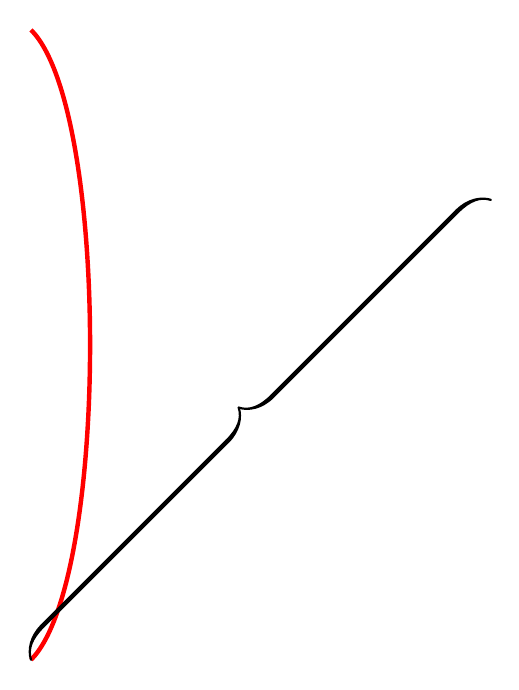
\begin{tikzpicture}
\draw[red,postaction={decorate,black},decoration={calligraphic brace,amplitude=4mm},ultra thick] (0,0) .. controls +(1,1) and +(1,-1) .. (0,8);
\end{tikzpicture}
\end{document}

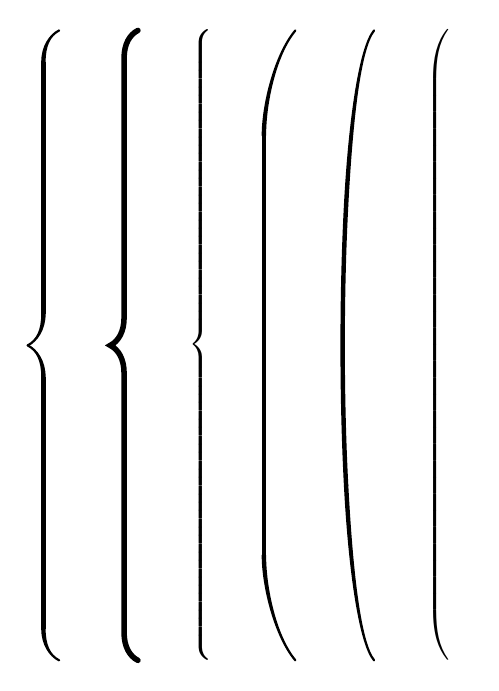
\begin{tikzpicture}
\draw[decorate,decoration={calligraphic brace,amplitude=4mm},ultra thick] (0,0) -- (0,8);
\draw[line width=2pt,decorate,decoration={brace,amplitude=10},line cap=round] (1,0) -- ++(0,8);
\node[anchor=south west,minimum height=8cm,outer sep=0pt,left delimiter=\{] (a) at (2,0) {};
\draw[decorate,decoration={calligraphic straight parenthesis,amplitude=4mm},ultra thick] (3,0) -- ++(0,8);
\draw[decorate,decoration={calligraphic curved parenthesis,amplitude=4mm},ultra thick] (4,0) -- ++(0,8);
\node[anchor=south west,minimum height=8cm,outer sep=0pt,left delimiter=(] (a) at (5,0) {};
\end{tikzpicture}
\end{document}
